\section{Natural Language Based CLI Framework}

\begin{figure}[h]
    \begin{center} 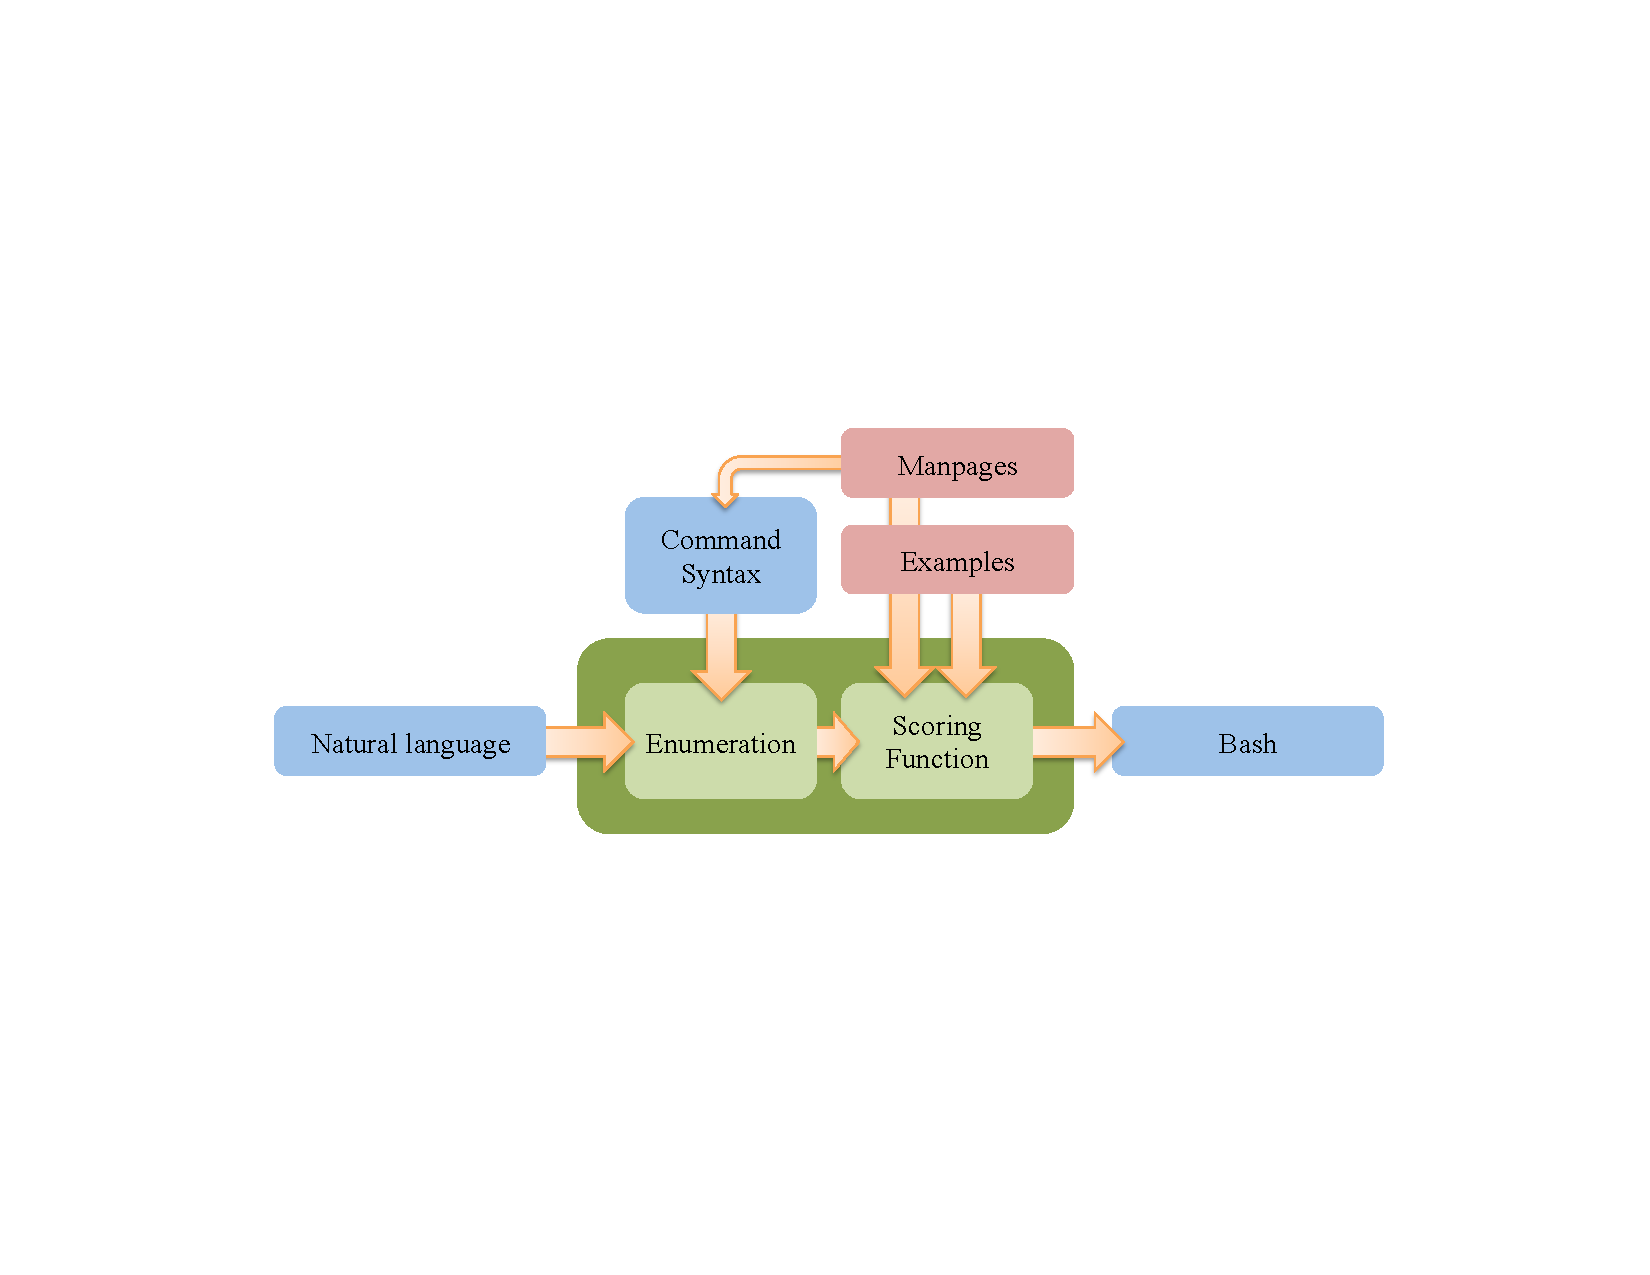
\includegraphics[width=4in]{architecture.pdf} \end{center}
    \caption{The overall architecture of our tool. Offline, the tool learns the
        valid syntax for common Bash commands using manpages. Both the manpages
        and a set of input-output examples are used to learn an appropriate
        scoring function. At runtime, the tool enumerates possible candidate
        programs using the learned syntax, scores them using the learned scoring
        function, and presents the top-ranked suggestions to the user.}
    \label{fig:arch}
\end{figure}

The natural language based command line interpreter we plan to develop consists of two key components: 1) an intermediate language to represent commands and
2) a semantic parser that maps natural language commands issued by users to this intermediate representation. Our initial pilot system is restricted to cover only file system operations, including file lookup, directory tree transformation, file content transformation, and file property modifications. We restrict the domain in the hope that it can be expressed with tractable logic and to reduce the degree of ambiguity in the natural language command. Section~\ref{subsec:represent} introduces the formal language design---the subset of Bash our tool supports---and section~\ref{subsec:parser} introduces the approach to train the semantic parser.

\subsection{Language Design}
\label{subsec:represent}
An ideal intermediate language for the CLI programs should be expressive enough so that it covers many interesting real world cases, concise enough for the synthesizer to efficiently synthesize, and extensible. \autoref{fig:lang} presents the syntax of the intermediate language.

\begin{figure}
\[
\begin{array}{rlll}
\multicolumn{3}{l}{\textbf{Program}}\\
\mathit{p} & := & \mathit{value} \\
    &  & \mathit{cmd}~\overline{\mathit{flag}}~\overline{\mathit{arg}} & \textrm{(Program)}\\
    &  & \mathit{p} ~\| ~\mathit{p} & \textrm{(Pipelined program)}\\
\mathit{value} & := & \mathsf{date} ~|~ \mathsf{filename} ~|~ ... & \textrm{(Primitive values)}\\
\mathit{arg} & := & \epsilon ~|~ \mathit{value} ~|~ \mathit{hole} & \textrm{(Arguments)}\\
\mathit{cmd}^{*} & := & \mathsf{find} ~|~ \mathsf{grep} ~|~ ... & \textrm{(Commands)}\\
\mathit{flag}^{*} & := & \epsilon ~|~ -f ~|~ -h ~|~ ... & \textrm{(Flags)}\\
~\\
\multicolumn{3}{l}{\textbf{Command Signature}}\\
\mathit{sig} & := & \mathsf{name}~\mathit{option}:\tau & \textrm{(Command signature)}\\
\mathit{option} &:= & \mathsf{flagname} & \textrm{(Command option)}\\
                &   & \mathsf{argname}[\tau]\\
                &   & \mathit{option}~\mathbf{or}~\mathit{option}\\
                &   & [ \mathit{option} ]\\
~\\
\multicolumn{3}{l}{\textbf{Rules}}\\
\mathit{rule}^{*} &:=& \mathsf{find}~f[\mathsf{File}] : \mathsf{File}\\
                  &  & \mathit{date}~\mathit{-d} : \mathsf{void}\\
                  &  & \mathit{date}~\mathit{-u} : \mathsf{Date}\\
                  &  & ...\\
~\\
\multicolumn{3}{l}{\textbf{Types}}\\
\tau_0 & := & \mathsf{void} ~|~ \mathsf{File} & \textrm{(Primitive types)}\\
       &     & |~ \mathsf{Date} ~|~ \mathsf{Permission} ~|~ \mathsf{Size} ~|~ ... \\
\tau & := & \tau_0 ~|~ \tau_0\rightarrow \tau_0 & \textrm{(Type)}
\end{array}
\]
\caption{Intermediate Language}
\label{fig:lang}
\end{figure}


\textbf{Program} defines how a program can be formed. A CLI program can refer to a value, call a primitive command, or pipeline two programs together.

The rest of the language are designed to help check well-formedness of a given CLI program. The command signature defines how a rule can be written, the rules (\textbf{Rule}) defines which primitive programs are valid. Then, with the help of the types in our program, we can check the type of a program $p$ to ensure that a command line program is well-formed.

Since the number of basic Linux commands and options is large even in domain-specific scenarios, it is difficult for a human designer to hand-code all of the generation rules. We plan to semi-automate this step by adding information extracted from the Linux man pages\footnote{\url{http://linux.die.net/man/}}. Extending our tool to handle new commands simply requires adding a new man page to the training data.

\subsection{Natural Language Command Interpreter}
\label{subsec:parser}
We train the natural language command interpreter using the Linux man pages, in addition to a small set of input/output pairs, each consisting of a natural language query and a command line program. The online forum StackOverflow has a large volume of input/output pairs. Unfortunately these conversations are noisy and only a handful of high-quality training pairs can be confidently extracted. In contarst, the Linux man pages are well formatted and contains rich natural language text that explains the usage of each command template and its possible arguments. We propose to use the command-explanation pairs extracted from man pages as additional signals to guide the search for high score rankings, thereby remedies the lack of example training pairs.

We use a linear feature function to score the natural language command to logical representation mappings. The following features are used:
\begin{itemize}\itemsep-1pt
	\item association of key words/phrases to partial expressions
	\item association between partial expressions (e.g. how often do they combined in valid commands)
	\item similarity of key words/phrases in the command to the man page explanation text of a partial expression
	\item complexity of the logical formulas and the commands generated from them.
\end{itemize}
We use the structured perceptron algorithm to learn weights of the scoring function from the example pairs. In each training iteration, we search for the top ranked logical form and update the weights based on its similarity to the ground truth logical form.
% We planned to extend learning into an interactive setting once the basic framework is developed.
